\documentclass[border=10pt]{standalone}

\usepackage{tikz}
\usepackage{tikzsymbols}
\usetikzlibrary{calc,patterns,shapes.geometric}

\def\centerarc[#1](#2)(#3:#4:#5){\draw[#1] ($(#2)+({#5*cos(#3)},{#5*sin(#3)})$) arc (#3:#4:#5);}

\begin{document}
	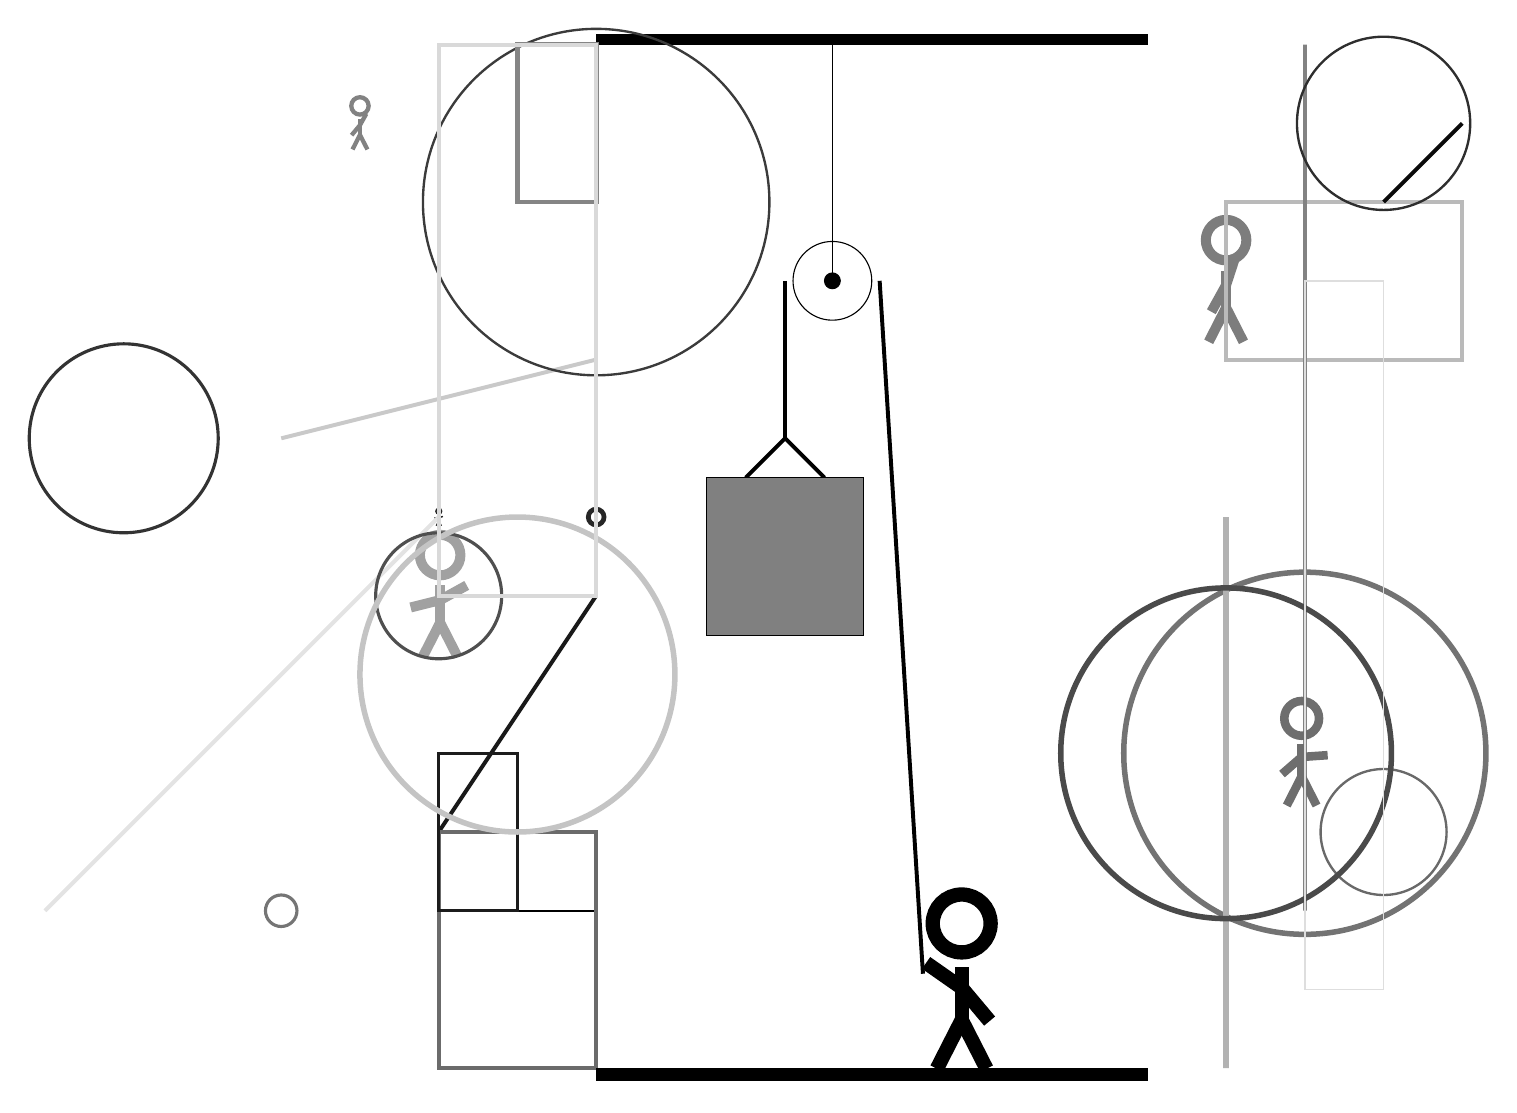
\begin{tikzpicture}
		%%%%% START %%%%%
		
		\draw[fill=black] (-2, 10) rectangle (5, 10.125);
		
		\draw (1, 7) circle (0.5);
		\draw[fill=black] (1, 7) circle (0.1);
		\draw (1, 10) -- (1, 7);
		
		\draw[line width=0.5mm] (-0.1, 4.5) -- (0.4, 5.0) -- (0.9, 4.5);
		\draw[fill=black!50] (-0.6, 4.5) rectangle (1.4, 2.5);
		
		\draw[line width=0.5mm] (0.4, 7) -- (0.4, 5.0);
		\centerarc[line width=0.5mm](1, 7)(0:180:0.6);
		\draw[line width=0.5mm](1.6, 7) -- (2.15, -1.8);
		
		\draw[line width=0.2mm, color=black!100] (-4, -1) rectangle (-2, -3);
		
		\draw [line width=0.3mm, color=black!59](8, 0) circle (0.8);
		\draw [line width=0.7mm, color=black!20](6, 4) circle (0.0);
		\node[line width=0.6mm, color=black!85] at (-4, 4) {\Strichmaxerl[1][4][16]};
		
		\draw[line width=0.5mm, color=black!90](-4, 0) -- (-2, 3);
		\draw[line width=0.5mm, color=black!58] (-4, -3) rectangle (-2, 0);
		\draw [line width=0.5mm, color=black!64](6, 6) circle (0.0);
		\draw [line width=0.7mm, color=black!55](7, 1) circle (2.3);
		\draw [line width=0.4mm, color=black!54](-6, -1) circle (0.2);
		\node[line width=0.2mm, color=black!51] at (6, 7) {\Strichmaxerl[7][61][72]};
		\draw[line width=0.5mm, color=black!21](-6, 5) -- (-2, 6);
		\draw[line width=0.5mm, color=black!11](-4, 4) -- (-9, -1);
		\draw [line width=0.4mm, color=black!80](-8, 5) circle (1.2);
		\draw [line width=0.6mm, color=black!85](-2, 4) circle (0.1);
		\node[line width=0.6mm, color=black!49] at (-5, 9) {\Strichmaxerl[3][50][61]};
		\draw[line width=0.4mm, color=black!89] (-3, 1) rectangle (-4, -1);
		
		\draw [line width=0.3mm, color=black!77](-2, 8) circle (2.2);
		\draw[line width=0.5mm, color=black!27] (6, 8) rectangle (9, 6);
		\draw[line width=0.7mm, color=black!30] (6, 4) rectangle (6, -3);
		
		\draw[line width=0.5mm, color=black!96](8, 8) -- (9, 9);
		\node[line width=0.7mm, color=black!37] at (-4, 3) {\Strichmaxerl[7][14][29]};
		
		\draw[line width=0.5mm, color=black!49] (7, -1) rectangle (7, 10);
		\draw [line width=0.7mm, color=black!71](6, 1) circle (2.1);
		\draw[line width=0.6mm, color=black!48] (-2, 10) rectangle (-3, 8);
		\draw [line width=0.3mm, color=black!82](8, 9) circle (1.1);
		\draw [line width=0.4mm, color=black!69](-4, 3) circle (0.8);
		\draw [line width=0.7mm, color=black!23](-3, 2) circle (2.0);
		\node[line width=0.6mm, color=black!57] at (7, 1) {\Strichmaxerl[6][41][4]};
		\draw[line width=0.2mm, color=black!13] (7, -2) rectangle (8, 7);
		
		\draw[line width=0.5mm, color=black!15] (-2, 3) rectangle (-4, 10);
		
		\node at (2.6, -1.9) {\Strichmaxerl[10][-35][-50]};
		
		\draw[fill=black] (-2, -3) rectangle (5, -3.15);
		
		%%%%% END %%%%%
	\end{tikzpicture}
\end{document}